\section{Discussion}
\label{sec:discussion}

\subsection{Public AI repositories}

There is no standard for the documentation and no standard for the usage.
It could be great to develop a standard
way to access AI models. This will allow to use more models from more different
repositories to give access to more people. For this paper we have tried to use
some repositories like below.

\begin{table}[H]
    \centering
    \caption{\label{tab:discussion}%
        Repositories not selected for this work
    }
    \begin{tabular}{lcccc}
      \toprule
      Repository & Mask Generation Model(s) \\
      \midrule
      PyTorch Hub & +50 \\
      Dinov2 & +10 \\
      Hailo.AI & 1 \\
      ModelZoo & 2 \\
      MicroSAM & +10 \\
      \bottomrule
    \end{tabular}
\end{table}

The lack of documentation, of APIs or of models available made it impossible to
use these repositories in WIPP. We hope to be able to integrate them into our
tool in the future.

\subsection{Documentation}

Documentation is also very important. Creating standard for AI model cards
could be great for the community.

In WIPP we have made decision by synthesizing the main AI model cards
already on the market:
\begin{itemize}
    \item Model Cards for Model Reporting, Google \cite{DBLP:journals/corr/abs-1810-03993}
    \item \href{https://huggingface.co/docs/hub/en/model-cards}{Model Cards, Hugging Face}
    \item \href{https://bioimage.io/docs/#/bioimageio_model_spec}{Fields to describe AI models, BioImage.IO}
    \item \href{https://github.com/tensorflow/model-card-toolkit}{Automates the generation of model cards, TensorFlow}
\end{itemize}




\def\firstellip{(1.6, 0) ellipse [x radius=2.7cm, y radius=1.5cm, rotate=50]}
\def\secondellip{(0.3, 1cm) ellipse [x radius=2.7cm, y radius=1.5cm, rotate=50]}
\def\thirdellip{(-1.6, 0) ellipse [x radius=2.7cm, y radius=1.5cm, rotate=-50]}
\def\fourthellip{(-0.3, 1cm) ellipse [x radius=2.7cm, y radius=1.5cm, rotate=-50]}

\begin{figure}[H]
\centering
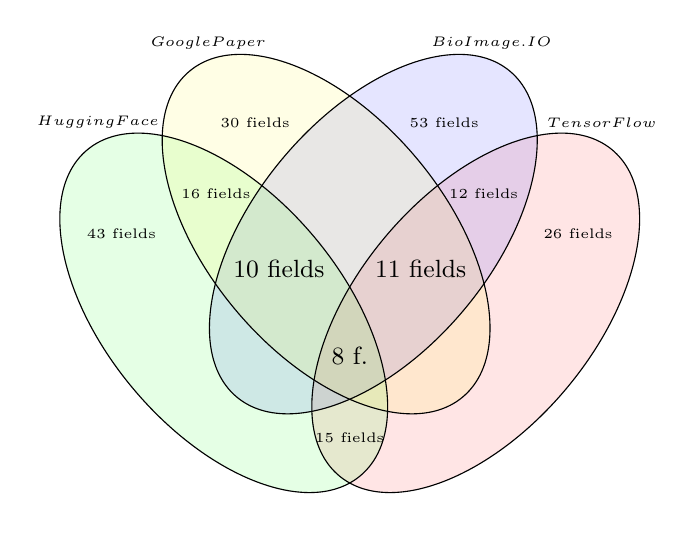
\begin{tikzpicture}

    \filldraw[fill=red,opacity=0.1] \firstellip;
    \filldraw[fill=blue,opacity=0.1] \secondellip;
    \filldraw[fill=green,opacity=0.1] \thirdellip;
    \filldraw[fill=yellow,opacity=0.1] \fourthellip;

    % TensorFlow (TF)
    \draw \firstellip node [label={[xshift=1.6cm, yshift=2.1cm] \tiny $TensorFlow$}] {};
    \draw node [label={[xshift=2.9cm, yshift=0.7cm] \tiny 26 fields}] {};

    % BioImage.IO (BI.IO)
    \draw \secondellip node [label={[xshift=1.5cm, yshift=2.1cm] \tiny $BioImage.IO$}] {};
    \draw node [label={[xshift=1.2cm, yshift=2.1cm] \tiny 53 fields}] {};

    % Hugging Face (HF)
    \draw \thirdellip node [label={[xshift=-1.6cm, yshift=2.1cm] \tiny $Hugging Face$}] {};
    \draw node [label={[xshift=-2.9cm, yshift=0.7cm] \tiny 43 fields}] {};

    % Google Paper (GP)
    \draw \fourthellip node [label={[xshift=-1.5cm, yshift=2.1cm] \tiny $Google Paper$}] {};
    \draw node [label={[xshift=-1.2cm, yshift=2.1cm] \tiny 30 fields}] {};

    % 
    \draw node [ label={ [xshift=-1.7cm,  yshift=1.2cm]   \tiny 16 fields} ] {};   % HF x GP
    \draw node [ label={ [xshift=1.7cm,   yshift=1.2cm]   \tiny 12 fields} ] {};   % BI.IO x TF
    \draw node [ label={ [xshift=0cm,     yshift=-1.9cm]  \tiny 15 fields} ] {};   % HF x TF
    \draw node [ label={ [xshift=-0.9cm,  yshift=0.2cm]   \small 10 fields} ] {};   % BI.IO x HF x GP
    \draw node [ label={ [xshift=0.9cm,   yshift=0.2cm]   \small 11 fields} ] {};   % BI.IO x TF x GP
    \draw node [ label={ [xshift=0cm,     yshift=-0.9cm]  \small  8 f.} ] {};   % HF x GP x BI.IO x TF

\end{tikzpicture}
\caption{Common field of different AI Model Cards} \label{fig:venn}
\end{figure}

This give us 8 fields that we want to keep to be as compatible as possible with
external tools. At the end we proposed an AI model card with 14 fields.

%\begin{itemize}
%    \item String: version
%    \item String: name
%    \item Date: date
%    \item String: framework
%    \item Map$\langle$String, String$\rangle$: trainingData
%    \item Map$\langle$String, String$\rangle$: trainingParameters
%    \item String: author
%    \item String: description
%    \item and more ...
%\end{itemize}

%For our needs, this works well, and
We manage to retrieve all this information automatically throughout the workflow.

%This proposal is not perfect and needs refinering.
The creation of a standard
would be a great opportunity for all the AI actors to think about what they
need.


%\begin{figure}[H]
%\centering
%\begin{tikzpicture}
%
%    \draw[draw=black] (-1.25,-1.25) rectangle ++(3.5, 3);
%    \filldraw[fill=red, opacity=0.1](0, 0) circle (1);
%    \filldraw[fill=blue, opacity=0.1](1, 0) circle (1);
%
%    \draw node [label={[xshift=0.5cm, yshift=-0.33cm] TP}] {};
%    \draw node [label={[xshift=0.5cm, yshift=1cm] TN}] {};
%    \draw node [label={[xshift=1.5cm, yshift=-0.33cm] FP}] {};
%    \draw node [label={[xshift=-0.5cm, yshift=-0.33cm] FN}] {};
%
%\end{tikzpicture}
%\caption{GT in red and PREDIC in blue} \label{fig:dice}
%\end{figure}



